% -----------------------------------------------------
% CHAPTER 1
% -----------------------------------------------------

\chapter{Week 1 \\ Practical Aspects of Deep Learning}







% - Setting up your Machine Learning Application --------------------------------

\section{Setting up your Machine Learning Application}

\subsection*{Train/Dev/Test Sets}

\begin{itemize}
    \item \textbf{Training set}: used to train the model
    \item \textbf{Dev/cross validation set}: used to evaluate the model and tune hyperparameters
    \item \textbf{Test set}: used to evaluate the model
\end{itemize}

\subsection*{Set Sizes}

How a data set is split into train/dev/test depends on the size of the data set. Here are some examples: 

\begin{tabular}[t]{|l|r|r|r|}
    \hline
    m & train & dev & test \\
    \hline
    $<10,000$ & $70$ & $30$ & \\
    \hline
    $<10,000$ & $60$ & $20$ & $20$\\
    \hline 
    $>1,000,000$ & $98$ & $1$ & $1$\\
    \hline
\end{tabular}

\subsection*{Mismatching train/test sets}

\begin{itemize}
	\item Do the training on one distribution of data that might be easier to gather, or consists of synthetic data, augmented data etc., then do testing on a different distribution.
	\item Test and dev should be from the same distribution.
    \item It may be OK to not use a test set, but just work with train \& dev cross validation.
\end{itemize}






% - Bias/Variance ---------------------------------------------------------------

\section{Bias \& Variance}

\begin{figure}[htbp] % 'htbp' is a placement specifier; it means "here, top, bottom, page"
    %\centering
    
    \begin{minipage}[t]{0.3\textwidth}
        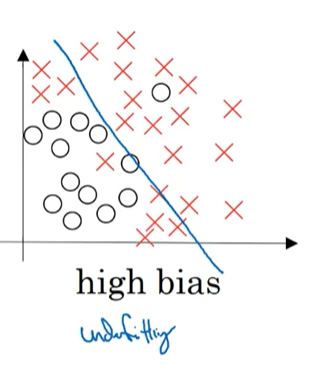
\includegraphics[width=\linewidth, valign=t]{images/high_bias.png}
    \end{minipage}
    \hfill % This will create horizontal space between the images
    \begin{minipage}[t]{0.3\textwidth}
        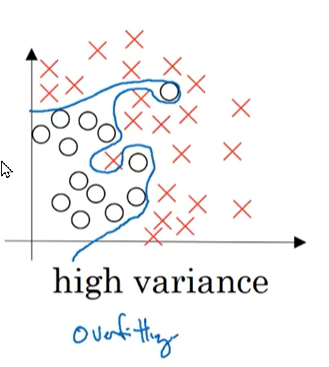
\includegraphics[width=\linewidth, valign=t]{images/high_variance.png}
    \end{minipage}
    \hfill
    \begin{minipage}[t]{0.3\textwidth}
        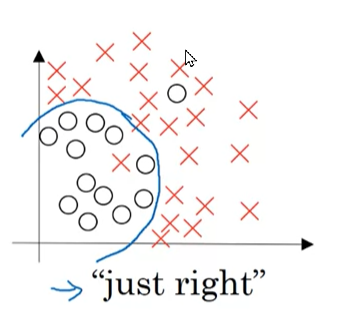
\includegraphics[width=\linewidth, valign=t]{images/low_b_v.png}
    \end{minipage}
    
\end{figure}


Given an optimal error of $0\%$

\begin{tabular}[t]{|l|l|l|l|l|}
    \hline
    Train Error & $1\%$ & $15\%$ & $15\%$ & $0.5\%$ \\
    \hline
    Dev Error & $11\%$ & $16\%$ & $30\%$ & $1\%$ \\
    \hline
    & 
    \begin{tabular}{l}
        High variance \\
        Overfitting
    \end{tabular}
    &
    \begin{tabular}{l}
        High bias\\
        Underfitting
    \end{tabular}
    &
    \begin{tabular}{l}
        High bias,\\ 
        variance
    \end{tabular}
    &
    \begin{tabular}{l}
        Low bias,\\ 
        variance
    \end{tabular}
    \\
    \hline
\end{tabular}

\begin{figure}[htbp] % 'htbp' is a placement specifier; it means "here, top, bottom, page"
    \begin{minipage}[t]{0.3\textwidth}
        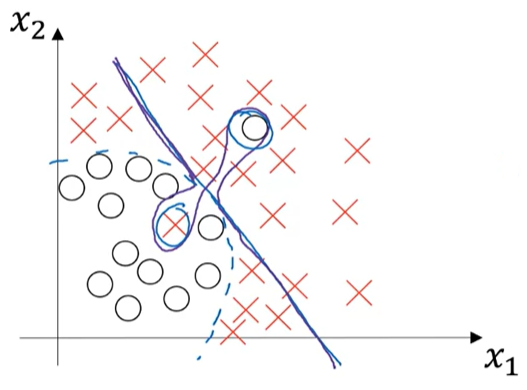
\includegraphics[width=\linewidth, valign=t]{images/high_b_v.png}
        \caption*{High bias, high variance}
        \label{fig:high_b_v}
    \end{minipage}
\end{figure}

This seems like a contrived example in two dimensions, but in higher dimensions its more plausible.

\subsection*{Basic Recipe for Machine Learning}

If high bias (underfitting):
\begin{itemize}
    \item bigger network
    \item train longer
    \item different NN architecture
\end{itemize}

If high variance (overfitting):
\begin{itemize}
    \item more data
    \item regularization
    \item different NN architecture 
\end{itemize}
    
Rinse and repeat until low bias \& variance.There's not much trade off between bias and variance in deep learning

\newpage





% -- Regularizing your Neural Network ------------------------------------------

\section{Regularizing your Neural Network}

\subsection*{Adding a Regularization Term}

\subsubsection*{Logistic regression}

\[ \underset{(w, b)}{min} \in J(w, b) \]
\[ w\in\mathbb{R}^{n_x}$, $b\in\mathbb{R} \]
\[ J(w,b)=\frac{1}{m} \sum_{i=1}^{m}\mathcal{L}(\hat{y}^{(i)}, y^{(i)}) \]

Add regularization (L2-regularization)
\[ \mathcal{J}(w,b)=\frac{1}{m} \sum_{i=1}^{m}\mathcal{L}(\hat{y}^{(i)}, y^{(i)})+ \frac{\lambda}{2m} \|w\|_2^2 \]

where
\[ \|w\|_2^2=\sum_{j=1}^{n_x}w_j^2=w^Tw \]


Add regularization (L1-regularization)

\[ \mathcal{J}(w,b)=\frac{1}{m} \sum_{i=1}^{m}\mathcal{L}(\hat{y}^{(i)}, y^{(i)})+ \frac{\lambda}{2m} \|w\|_1 \]

where
\[ \|w\|_1 = \sum_{j=1}^{n_x}|w_j| \]

L1-regularization can lead to w becoming sparse

$\lambda$ is called the regularization parameter

We could add a regularization term on b as well, but has little effect compared to the w-based term.

\subsubsection*{Neural Network}

Add regularization term over all layers' parameters:
\[ 
    \mathcal{J}(w^{[1]}, b^{[1]}, \ldots, w^{[L]} , b^{[L]} )=\frac{1}{m} \sum_{i=1}^{m}\mathcal{L}(\hat{y}^{(i)}, y^{(i)})+ 
    \frac{\lambda}{2m}\sum_{l=1}^L\|w^{[l]}\|_F^2 
\]

$w$ is a $(n^{[l]} , n^{[l-1]})$ matrix, and the "L2-norm" of a matrix is called the Frobenius norm. 
For a layer $l$ the norm is:
\[ \|w^{[l]}\|_F^2= \sum_{i=1}^{n^{[l-1]}} \sum_{j=1}^{n^{[l]}}({w_{ij}}^{[l]})^2 \]

\subsubsection*{Gradient descent with regularization}

\begin{align}
    dw^{[l]}= & (\text{from backprop})+ \frac{\lambda}{m} w^{[l]} \\
    w^{[l]} = & w^{[l]} - \alpha dw^{[l]} \\
            = & w^{[l]} - \alpha( (\text{from backprop}) + \frac{\lambda}{m}w^{[l]} ) \\
            = & w^{[l]} - \alpha \frac{\lambda}{m} w^{[l]} - \alpha(\text{from backprop})
\end{align}


The second term has the effect of reducing the size of $w$ slightly, 
which is why this regularization is also called "weight decay."

\subsubsection*{How does regularization prevent overfitting?}

Intuition: With a large value for $\lambda$, the $w^{[i]}$  will be brought to $\approx${0}, 
in effect zeroing out the effect of some nodes in the network, bringing the variance down. 
In practice, the weights won't be 0, but the values will be smaller.
\[ \lambda \uparrow \implies w^{[l]} \downarrow\]

so then
\[ z^{[l]} = w^{[l]}  a^{[l-1]} + b \]

will be small, and so the activation function
\[ g(z)=tanh(z) \]

will be close to linear for those values of $z$, and the network will behave more like a linear network: 

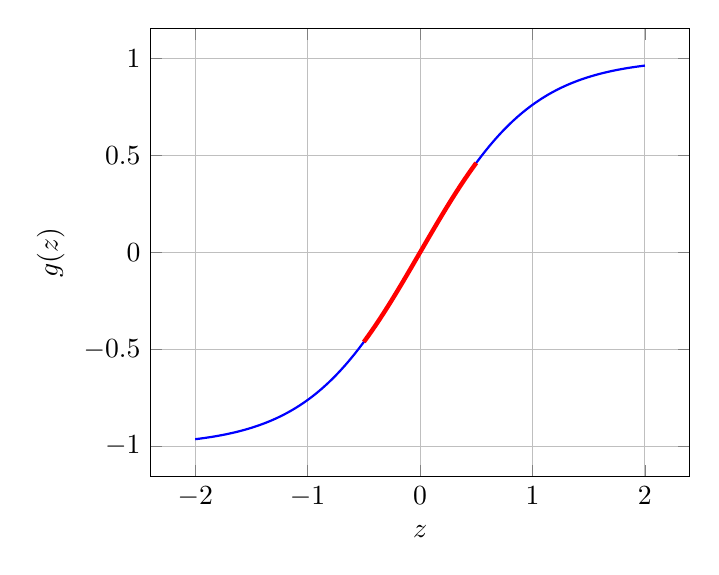
\begin{tikzpicture}
    
    \begin{axis}[
        xlabel={\( z \)},
        ylabel={\( g(z) \)},
        grid=major,
        %title={tanh activation function, \( g(z) = \tanh(z) \)},
        domain=-2:2,
        samples=100,
    ]
    \addplot[blue, thick] {tanh(x)};
    \addplot[red, ultra thick, domain=-0.5:0.5] {tanh(x)};

    %\legend{\( g(z) = \tanh(z) \), almost linear part}
    \end{axis}
\end{tikzpicture}




\newpage

\subsection*{Dropout regularization}

\begin{figure}[htbp]
    \begin{minipage}[t]{\textwidth}
        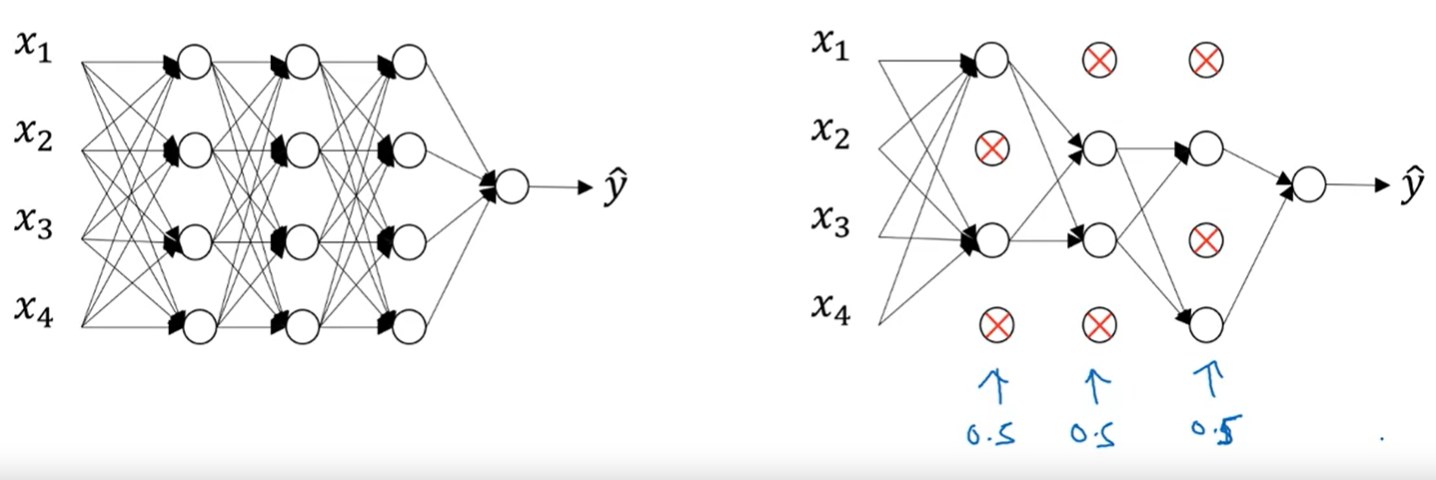
\includegraphics[width=\linewidth, valign=t]{images/dropout.png}
        \caption*{Dropout}
    \end{minipage}
\end{figure}

\subsubsection*{Implementing dropout}

\begin{algorithm}[H]
    \caption*{Inverted dropout}
    \begin{algorithmic}[1]
        \BlockComment{Probability of keeping a node active}
        \State $keep\_prob = \ldots$
        \BlockComment{Vector of bools}
        \State $d^{[l]} = np.random.rand(a^{[l]}.shape[0], a^{[l]}.shape[1]) < keep\_prob$
        \BlockComment{Keep the nodes where d is True only}
        \State $a^{[l]} = np.multiply(a^{[l]}, d^{[l]})$
        \BlockComment{Scale the result}
        \State $a^{[l]} /= keep\_prob$
    \end{algorithmic}
\end{algorithm}

The last line is to scale a3 back to the expected size when used in the activation function, 
and also keeps it in line with the size used in inference, when dropout is not employed.

Intuition: Can't rely on any one feature, so have to spread out the weights $\implies$ smaller weights, 
similar to L2 regularization.

It may be a good idea to have different values for $keep\_prob$ for different layers:
\begin{itemize}
    \item low for the larger ones (many inputs and outputs) where overfitting is more likely a risk, 
    \item higher for others, up to 1.0 (no dropout) for the smallest layers. 
\end{itemize}


\textbf{Downsides}:
\begin{itemize}
    \item increases the number of hyperparameters to find good values for.
    \item the cost function $\mathcal{J}(w, b)$ is no longer well defined. 
        This means the graph of loss x training iteration becomes less meaningful.
\end{itemize}

\newpage

\subsection*{Other regularization methods}

\subsubsection*{Data augmentation}

If you can't collect more data, try augmenting existing data with variations, 
e.g. by flipping or random rotation, distortion and/or cropping of images. 
This will not add as much information as collecting more data,
but will give your algorithm more data and therefore sort of regularize it and reduce over fitting.

\begin{figure}[htbp]
    \begin{minipage}[t]{\textwidth}
        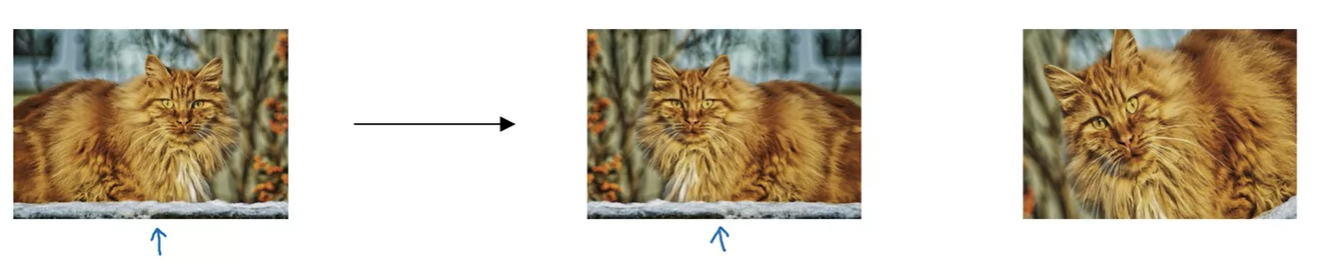
\includegraphics[width=\linewidth]{images/augmented_catpic.png}
    \end{minipage}
\end{figure}

\subsubsection*{Early stopping}

Stopping when dev set error is at a minimum.

\begin{figure}[htbp]
    \begin{minipage}[t]{\textwidth}
        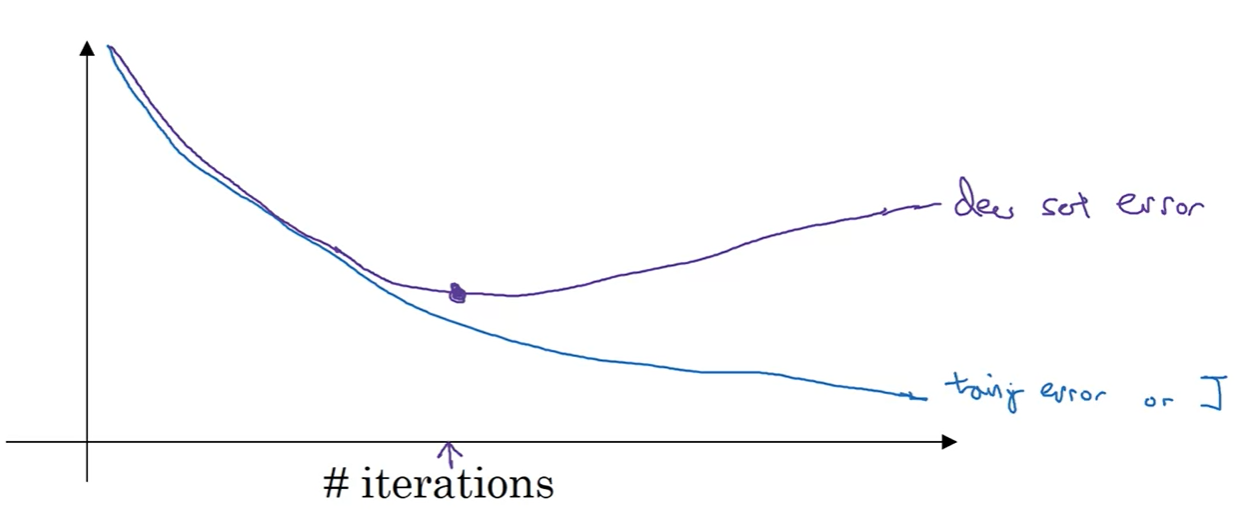
\includegraphics[width=\linewidth]{images/early_stopping.png}
    \end{minipage}
\end{figure}

When you haven't run many iterations, $w\approx0$. During training, the values of w will increase,
so on the right part of the x-axis above, values for w will be large. At the mid point in the graph, 
the value for $\|w\|_F^2$  will be ``mid-sized''. So by picking this version of the network, 
you will get a network with smaller weights, much like one trained with L2-regularization.

\textbf{Downside}: Breaking orthogonality between optimizing $\mathcal{J}(w, b)$ and avoiding overfitting. 
In ML, we can otherwise view these two concepts as orthogonal:

\begin{itemize}
	\item Optimize cost function $\mathcal{J}(w, b)$, using
	\begin{itemize}
		\item Gradient descent
		\item Adam
		\item ...
    \end{itemize}
	\item Avoid overfitting by
    \begin{itemize}
        \item regularization
		\item more data
		\item ...
    \end{itemize}
\end{itemize}

%\newpage





% -- Setting Up your Optimization Problem ---------------------------------------

\section{Setting Up your Optimization Problem}

\subsection*{Normalizing Inputs}

\begin{figure}[htbp]
    \centering
    \begin{minipage}[t]{0.6\textwidth}
        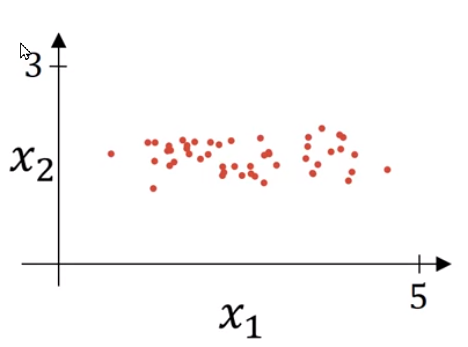
\includegraphics[width=\linewidth]{images/data_not_normalized.png}
    \end{minipage}
\end{figure}


\begin{tabular}{c|c}

    Subtract the mean: &
    Normalize variance: \\

    & \\

    \mbox{$\displaystyle \mu = \frac{1}{m} \sum_{i=1}^m x^{(i)} $} &
    \mbox{$\displaystyle \sigma^2 = \frac{1}{m} \sum_{i=1}^{m} (x^{(i)} - \mu)^2 $} \\

    & \\

    \fbox{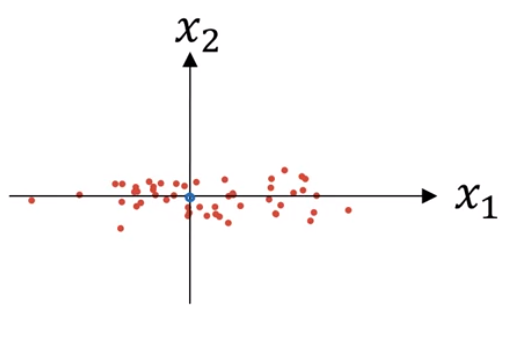
\includegraphics[width=0.4\textwidth]{images/data_mean_subtracted.png}} &
    \fbox{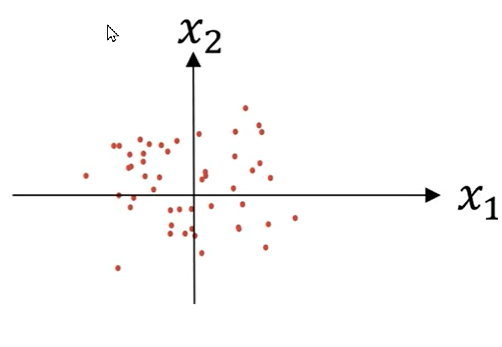
\includegraphics[width=0.4\textwidth]{images/data_normalized.png}} \\

    plot of $x - \mu$ &
    plot of $\frac{x - \mu}{\sigma}$ \\

    & \\

\end{tabular}

Scale the test set in the same way as the training set, with the same values for $\sigma$ and $\mu$.

\newpage

\subsection*{Why Normalize inputs?}

Plotting the cost function 

\[ \mathcal{J}(w, b)= \frac{1}{m} \sum_{i=1}^m \mathcal{L}(\hat{y}^{(i)}, y^{(i)}) \]

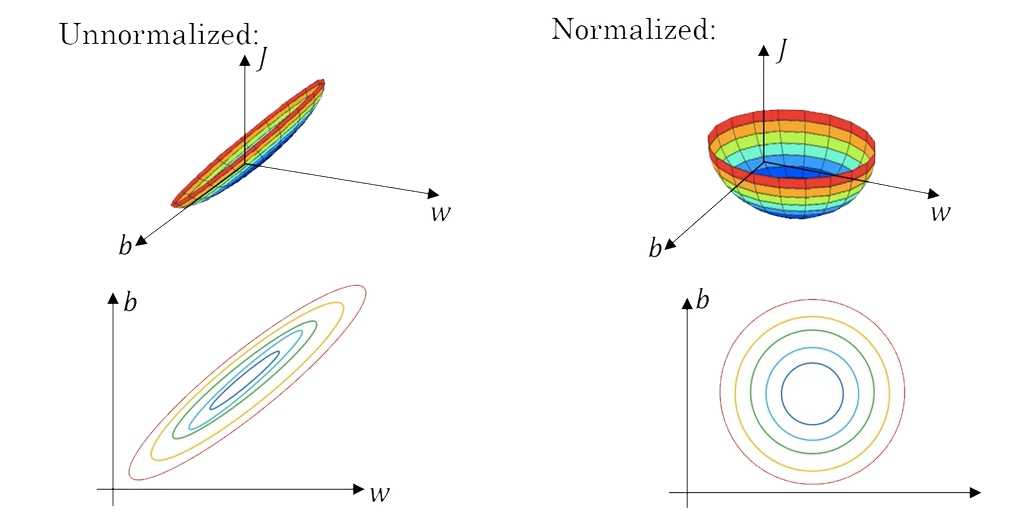
\includegraphics{images/normalized_cost_function.png}

In the non-normalized case, we may need a very small learning rate to avoid gradient descent jumping around all over the place,
whereas in the normalized case we can use a larger learning rate and the network can converge faster without oscillating:

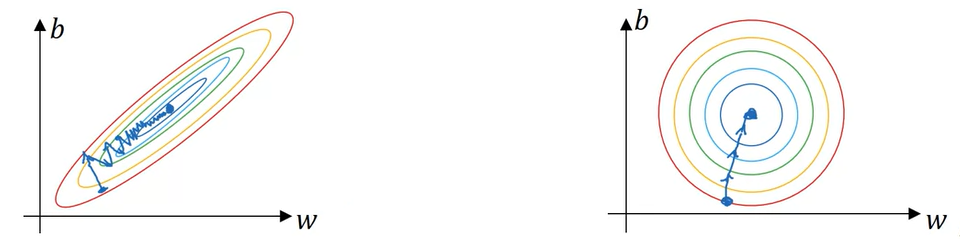
\includegraphics{images/normalized_gd.png}

\subsection*{Vanishing or Exploding Gradients}

During training of a deep network, gradients may grow exponentially large or small, making training difficult.

Example:

\begin{tikzpicture}[
    >={Latex[scale=1.5]},
    % Define the style for the nodes
    xory/.style={circle, minimum size=0.8cm, inner sep=0pt},
    neuron/.style={circle, draw=black, minimum size=0.8cm, inner sep=0pt},
    layer/.style={anchor=center, nodes=neuron, node distance=0.8cm}
]

% Input layer
\node[xory] (x1-1) {$x_1$};
\node[xory, below=of x1-1] (x1-2) {$x_2$};

% Hidden layers
\foreach \i [remember=\i as \lasti (initially 1)] in {2,...,8} {
    \node[neuron, right=0.8cm of x\lasti-1] (x\i-1) {};
    \node[neuron, below=of x\i-1] (x\i-2) {};
    \foreach \j in {1,2} {
        \foreach \k in {1,2} {
            \draw[->] (x\lasti-\k) -- (x\i-\j);
        }
    }
}

% Output layer
\node[neuron, right=0.8cm of x8-1, yshift=-0.8cm] (output) {};
\foreach \j in {1,2} {
    \draw[->] (x8-\j) -- (output);
}

\node[xory, right=0.8cm of output] (y-hat) {$\hat{y}$};
\draw[->] (output) -- (y-hat);

\end{tikzpicture}


This network has weights 
\[ w^1, w^2, \ldots, w^L \]

For the example we use a linear activation function
\[ g(z)=z \]

and set
\[ b^{[l]}=0 \]

Then we will have
\[ 
    \hat{y} = w^{[L]}w^{[L-1]} \times \ldots \times w^{[3]} w^{[2]} w^{[1]} x = w^{[L]} ( \prod_{l=1}^{L-1}w^{[l]})?x
\]

Now if
\[ 
    w^{[l]} =
    \begin{pmatrix}
        1.5 & 0 \\
        0 & 1.5 
    \end{pmatrix}
\]

Then for $\hat{y}$, the factor
\[
    \prod_{l=1}^{L-1}w^{[l]} = 
    \begin{pmatrix}
        1.5^{L-1} & 0 \\
        0 & 1.5^{L-1} 
    \end{pmatrix}
\]
and for large L, $1.5^{L-1}$ will become very large, and $\hat{y}$ will become very large.

Similarly, if we have
\[ 
    w^{[l]} =
    \begin{pmatrix}
        0.5 & 0 \\
        0 & 0.5 
    \end{pmatrix}
\]

Then for $\hat{y}$, the factor
\[
    \prod_{l=1}^{L-1}w^{[l]} = 
    \begin{pmatrix}
        0.5^{L-1} & 0 \\
        0 & 0.5^{L-1} 
    \end{pmatrix}
\]
and for large L, $0.5^{L-1}$ will become very small, and $\hat{y}$ will become very small.

So we have ($I$ being the identity matrix) that if
\[ w^{[l]} > I, \text{then with a deep network the activations can explode} \]
\[ w^{[l]} < I, \text{then with a deep network the activations can vanish} \]

A similar argument can be used to show that the derivatives or gradients will also increase 
or decrease exponentially as a function of the number of layers.


\subsection*{Weight Initialization for Deep Networks}

\begin{tikzpicture}[
    >={Latex[scale=2]},
    % Define the style for the nodes
    xory/.style={circle, minimum size=0.8cm, inner sep=0pt},
    neuron/.style={circle, draw=black, minimum size=0.8cm, inner sep=0pt},
    layer/.style={anchor=center, nodes=neuron, node distance=0.8cm}
]

\node[xory] (x1) {$x_1$};
\node[xory, below=0.7cm of x1] (x2) {$x_2$};
\node[xory, below=0.7cm of x2] (x3) {$x_3$};
\node[xory, below=0.7cm of x3] (x4) {$x_4$};
\node[neuron, right=2cm of x2, yshift=-0.7cm] (n1) {};
\node[xory, below=0.5cm of n1] (formula) {$a=g(z)$};
\node[xory, right=1.5cm of n1] (y1) {$\hat{y}$};

\draw[->] (x1) -- (n1);
\draw[->] (x2) -- (n1);
\draw[->] (x3) -- (n1);
\draw[->] (x4) -- (n1);
\draw[->] (n1) -- (y1);
    
\end{tikzpicture}


\[ z = w_1 x_1 + w_2 x_2 + \ldots + w_n x_n \]

so when $n \uparrow$, we want $w_i \downarrow$, in order not to have z grow too large.

One way of doing this is to make

\[ Var(w)= \frac{1}{n} \]

Do this by setting

\[ 
    w^{[l]} = 
    [rand(0 \ldots 1)] \times \sqrt{\frac{1}{n^{[l-1]}}} 
\]

where $[rand(0 \ldots 1)]$ is a random number between 0 and 1. This is called Xavier-initialization, 
and works well for the $tanh(z)$ activation function.

If using the ReLU activation function, using

\[ 
    w^{[l]} = 
    [random\ weight\ matrix] \times \sqrt{\frac{2}{n^{[l-1]}}} 
\]

has been found to work slightly better.

Another version is

\[
    w^{[l]} =
    [random\ weight\ matrix] \times \sqrt{\frac{2}{n^{[l-1]}+ n^{[l]}}}
\]

This could be made part of the hyperparameters to tune, but it's not the most important one.


\newpage



\subsection*{Gradient Checking}

Take all parameters $W^{[1]} , b^{[1]}, \ldots, W^L, b^L$  and reshape into a big vector $\theta$.

You will now have a cost function $\mathcal{J}(\theta)$

In the same way, gather all gradients $dW^{[1]} , db^{[1]}, \ldots, dW^L, db^L$ and reshape into a big vector $d\theta$.

We can now set

\[ 
    d\theta_{approx}^{[i]} = 
    (
        \mathcal{J}(\theta_1, \ldots, \theta_i + \epsilon, \ldots) 
        - 
        \mathcal{J}(\theta_1, \ldots, \theta_i - \epsilon, \ldots)  
    ) 
    / 
    2\epsilon
\]

We then do

\begin{algorithm}
    \caption*{Gradient Checking}
    \begin{algorithmic}[1]
        \Function{Check}{$d\theta_{approx}, d\theta, \epsilon$}
            \State \Return $\frac{||d\theta_{approx} - d\theta||_2}{||d\theta_{approx}||_2 + ||d\theta||_2} < \epsilon$
        \EndFunction

        \Statex
        
        \For {$i = 1$ to $n$}
            \State $Ok \gets$ \Call{Check}{$d\theta_{approx}^{[i]}, d\theta^{[i]}, 10^{-7}$}
        \EndFor
    \end{algorithmic}
\end{algorithm}		


\subsection*{Grad Check Implementation Notes}
\begin{itemize}
	\item Don't use in training - only to debug
	\item If grad check fails, look at the different components of $\theta$ to try to identify the bug. E.g. is it $dW$ or $db$ that is the problem?
	\item Remember the regularization term.
	\item Doesn't work with dropout.
	\item Run after random initialization (small $W, dW$), then again later after training for a while (larger $W, dW$). Errors might not show when the gradient is small.
\end{itemize}


